\section{Results--symmetry suppression theory}

%\subsection{Treatment of parity}
%The theoretical treatment of parity under $l$ and $j$-coupling is shown. The program AReTDoG as an implementation of this and its agreement with \cite{karlsson} is discussed.

%\subsection{Symmetry suppression theory} \label{sec:suppression}
%The first-order perturbation treatment of selection rules and its applicability to low-to-high symmetry systems is shown.

In our research, we tested the following hypothesis: \textit{Symmetry elevation effects are caused by transformation properties of the bulk symmetry.} Since the bulk symmetry group $T_d$ contains the structure symmetry $C_{3v}$ as a subgroup, it is a natural suspect for a source  of \textit{approximate} symmetries, since it limits the true symmetry of the system.

The theoretical basis for particular excitons enjoying symmetry transformations from the bulk symmetry is built on their localisation within the QD. If the envelope functions $\Upsilon_i$ of every fermion in an exciton complex are localised near the centre of the QD, any bulk-symmetry transformation should also be a symmetry transformation of the exciton wavefunction. With every QD border the envelope functions approach, more approximate symmetry transformations vanish, until, when an exciton has significant probability to measure one or more of its fermions around the entire edge of the QD, it fully probes the structure symmetry.

\subsection{Perturbative analysis of selection rules}
Suppose now we have a system described by a Hamiltonian $\hat{H}$ equipped with a group of symmetries $G$. Let us construct a Hamiltonian $\hat{H}_+$ which is equipped with a group of symmetries $G_+$ such that $G<G_+$ and $\hat{H}$ can be modelled as a perturbation of $\hat{H}_+$ like so:
	$$\hat{H}=\hat{H}_+ + \lambda \hat{H}',\qq{where}\lambda\ll 1$$
	For an exciton with its wavefunction localised in the centre of the QD, $\hat{H}$ is the true Hamiltonian, and $\hat{H}_+$ is the Hamiltonian of a smaller QD inscribed into the true QD with a higher symmetry.
	\subsubsection{Elevated symmetry component of an energy eigenstate}
	Let us denote the eigenstates of the Hamiltonians $\hat{H},\hat{H}_+$ as $\ket{E_i;n}$ and $\ket{E^+_{i'};n'}$ respectively, where $n, n'$ are the degeneracy labels. Disregarding accidental degeneracy, we know that every set of degenerate energy levels forms a basis of (i.e. transforms according to) an irrep of the respective symmetry group:
	$$\mqty(\ket{E_i;1}\\\ket{E_i;2}\\\vdots\\\ket{E_i;d_i})\mbox{ forms a basis to }\Gamma^{(G)}_{r(i)}; \mqty(\ket{E^+_{i'};1}\\\ket{E^+_{i'};2}\\\vdots\\\ket{E^+_{i'};d^+_{i'}})\mbox{ forms a basis to }\Gamma^{\left(G_+\right)}_{r^+(i')}$$
	where $d_i, d^+_{i'}$ specify the total degeneracies of the energy levels and $r,r^+$ are some functions which map energy levels onto irreps.
	Under a first-order perturbation of a set of degenerate eigenstates, the distance of the new states from the subspace $\mathcal{D}^+$ spanned by the degenerate eigenstates goes like $O(\lambda)$. Therefore, if $\ket{E_i;n}$ arises from perturbing a degenerate subspace of energy $E^+_j$, there exists an unnormalized vector $\ket{E^+_j;P}\in\mathcal{D}^+_j$ for which
	\begin{eqnarray*}
	\frac{\braket{E_i;n}{E^+_j;P}}{\abs{\braket{E^+_j;P}{E^+_j;P}}^{1/2}}&=&1-O(\lambda)\\
	\qq{where} \braket{E^+_j;P'}{E_i;n}&=&\braket{E^+_j;P'}{E^+_j;P}
	\qq{for all} \ket{E^+_j;P'}\in\mathcal{D}^+
	\end{eqnarray*}
	We can construct a state satisfying these conditions by projecting the perturbed eigenstate onto the original degenerate subspace:
	\begin{eqnarray*}
	\hat{P}^+_j&=&\sum_{m=1}^{d^+_j}\dyad{E^+_j;m}{E^+_j;m}\\
	\ket{E^+_j;P}&=&\hat{P}^+_j\ket{E_i;n}=\sum_{m=1}^{d^+_j}\ket{E^+_j;m}\braket{E^+_j;m}{E_i;n}
	\end{eqnarray*}
	Now we can express a general eigenstate of $\hat{H}$ as a superposition of an eigenstate of $\hat{H}^+$ with a norm that goes like $1-O(\lambda)$ and a remainder. We normalize the components and introduce superposition coefficients:
	\begin{equation}
	\ket{E_i;n}=c_{ES}\ket{E^+_j;ES}+c_R\ket{R}
	\end{equation}
	where the \textit{elevated symmetry component} is defined as
	\begin{eqnarray*}
	\ket{E^+_j;ES}&=&\ket{E^+_j;P}\abs{\braket{E^+_j;P}{E^+_j;P}}^{-1/2}\\
	&=&\ket{E^+_j;P}\left(\sum_{m=1}^{d^+_j}\abs{\braket{E^+_j;m}{E_i;n}}^2\right)^{-1/2}\\
	c_{ES}&=&\braket{E^+_j;ES}{E_i;n}\\
	&=&\sqrt{\sum_{m=1}^{d^+_j}\abs{\braket{E^+_j;m}{E_i;n}}^2}\\
	&\sim& 1-O\left(\lambda\right)
	\end{eqnarray*}
	and the \textit{residual component} then becomes
	\begin{eqnarray*}
	\ket{R}&=&c_R^{-1}\left(\ket{E_i;n}-c_{ES}\ket{E^+_j;ES}\right)
	\end{eqnarray*}
	By demanding norm 1, we obtain:
	\begin{eqnarray*}
	1&=&c_R^{-2}\left(\braket{E_i;n}{E_i;n}+c_{ES}^2\braket{E^+_j;ES}{E^+_j;ES}-2c_{ES}\braket{E_i;n}{E^+_j;ES}\right)\\
	c_R&=&\sqrt{1-c_{ES}^2}\\
	&\sim & O(\lambda)\\
	\ket{R}&=& \left(1-c_{ES}^2\right)^{-1/2}\left(\ket{E_i;n}-c_{ES}\ket{E^+_j;ES}\right)
	\end{eqnarray*}
	\subsubsection{Selection rules for the elevated symmetry component}
	Consider now two eigenstates of $\hat{H}$ at different energy levels, $\ket{E_i;n_i}$, $\ket{E_f;n_f}$. If we perturb the system with an interaction Hamiltonian $\hat{H}'$, the rate of transition between these two states is given by Fermi's golden rule
	$$\Gamma_{\ket{E_i;n_i}\to \ket{E_f;n_f}}=\frac{2\pi}{\hbar}\abs{\mel{E_f;n_f}{\hat{H}'}{E_i;n_i}}^2$$
	Since the energy levels may be degenerate, the full transition rate between the two sets of degenerate states becomes
	$$\Gamma_{E_i\to E_f}=\sum_{n_i=1}^{d_i}\sum_{n_f=1}^{d_f}\Gamma_{\ket{E_i;n_i}\to \ket{E_f;n_f}}$$
	Let the energy levels $E_i,E_f$ be chosen such that the direct product $\Gamma^{(G)}_{r(i)}\otimes \Gamma^{(G)}_{\hat{H}'}\otimes \Gamma^{(G)}_{r(f)}$ contains the identity irrep of $G$, and hence the matrix elements do not vanish due to the selection rule. Let us now decompose the two eigenstates into elevated symmetry and residual components:
	\begin{eqnarray*}
	\ket{E_i;n_i}&=&c_{ES}^i\ket{E_{i'}^+;ES}+c_R^i\ket{R_i}\\
	\ket{E_f;n_f}&=&c_{ES}^f\ket{E_{f'}^+;ES}+c_R^f\ket{R_f}
	\end{eqnarray*}
	where $E_{i'}^+,E_{f'}^+$ denote the energy levels of the high-symmetry Hamiltonian $\hat{H}^+$ which get perturbed into $E_i,E_f$ respectively.
	
	Let us now calculate the matrix element under the interaction Hamiltonian:
	\begin{eqnarray*}
	&&\mel{E_f;n_f}{\hat{H}'}{E_i;n_i}=\\
	&&\left(c_{ES}^f\right)^* c_{ES}^i \mel{E_{f'}^+;ES}{\hat{H}'}{E_{i'}^+;ES}+\left(c_{ES}^f\right)^* c_R^i \mel{E_{f'}^+;ES}{\hat{H}'}{R_i} + \\
	&&\left(c_{R}^f\right)^* c_{ES}^i\mel{R_f}{\hat{H}'}{E_{i'}^+;ES} + \left(c_{R}^f\right)^* c_R^i \mel{R_f}{\hat{H}'}{R_i}
	\end{eqnarray*}
	We know that $\left(c_{R}^f\right)^* c_R^i$ goes like $O\left(\lambda^2\right)$, and hence we will disregard the corresponding term. There are now two possibilities for what may occur:
	\begin{enumerate}
	\item \textit{The elevated symmetry matrix element does not vanish.} If $\Gamma^{\left(G_+\right)}_{r^+(i')}\otimes \Gamma^{\left(G_+\right)}_{\hat{H}'}\otimes \Gamma^{\left(G_+\right)}_{r^+(f')}$ contains the identity irrep of $G_+$, the leading term matrix element does not vanish, and forms the main contribution to the total matrix element.
	\item \textit{The elevated symmetry matrix element vanishes.} If $\Gamma^{\left(G_+\right)}_{r^+(i')}\otimes \Gamma^{\left(G_+\right)}_{\hat{H}'}\otimes \Gamma^{\left(G_+\right)}_{r^+(f')}$ does not contain the identity irrep of $G_+$, the leading term matrix element vanishes due to the selection rule (since it must transform as a scalar). The only non-zero terms are now the cross-terms, which both go like $O(\lambda)$, and the transition rate goes like $O(\lambda^2)$. Hence, even though these spectral lines are not fully forbidden by the selection rule, they are reduced by an order of magnitude (and vanish in first order) due to their high partial symmetry--this is symmetry suppression.
	\end{enumerate}

\subsection{Localisation of pure-heavy-hole excitons in the bulk}
The shape of the exciton wavefunctions is not well-understood, as calculating them is highly non-trivial. However, we can state qualitative arguments that describe the localisation of fermions in the QD approximately. For this, we will use the results from Sec. \ref{sec:envelopes} to treat the fermion envelope functions $\Upsilon_i$ as a Coulomb-interacting many-body system in a finite potential well. This highly approximate method will provide the justification for our expectation of some excitons being highly localised in the bulk of the QD.

Firstly, for a single particle in a finite potential well, we shall inquire on the role of the effective mass $m^*$ in the tunnelling of the wavefunction into the edges of the well, which probes the structure symmetry. As shown e.g. by Landau in \cite[p. 64]{landau}, the attenuation coefficient is proportional to $\sqrt{m^*}$ for $1$D wells. This result is readily generalised for $3$D systems of arbitrary shape, since in the region outside the well, the Schrödinger equation has the form
\begin{equation}
\left(\frac{\hat{p}}{\sqrt{2m^*}}\right)^2\ket{\Upsilon} = (E-V)\ket{\Upsilon}
\end{equation}
where $V>E$ is the depth of the potential well, larger than the particle energy, since the particle is constrained within the QD. We see that the sign of $E-V$ is negative. Since the particle is free in the regime outside of the potential well, we expect it to be (approximately) an eigenfunction of $\hat{p}$ as well as $\hat{H}$, especially if the shape of the potential well boundary in three dimensions is smooth. Then the eigenvalue of $\hat{p}$ must be purely imaginary to match the sign on both sides, and proportional to $\sqrt{m^*}$ for the attenuation coefficient in the spatial dependence to be of dimension $\unit{m}^{-1}$. This allows us to conclude that fermions with high effective mass (such as heavy holes with $m^*_{hh}\approx 0.5m_e$) will be more strongly localised in the centre of the QD bulk than fermions with low effective mass (such as electrons with $m^*_e\approx 0.059m_e$ and light holes with $m^*_{lh}\approx 0.076m_e$). \textit{Note.} The effective masses were calculated for $\text{In}_{0.10}\text{Ga}_{0.90}\text{As}$ with the formulas provided by Goldberg and Schmidt in \cite[p. 62]{semiconductor_handbook}. These formulas are stated for $T=\SI{300}{\kelvin}$, but we do not expect the effective masses to vary between $T=\SI{30}{\kelvin}$ and $\SI{300}{\kelvin}$ significantly for this qualitative argumentation, as the fact that $m_e^*$ and $m_{lh}^*$ are of the same order of magnitude and $m_{hh}^*$ is larger by an order of magnitude should remain true. This leads us to a hypothesis that single light holes and single electrons probe the structure symmetry, but single heavy holes are localised in the centre of the QD and undergo symmetry elevation to the bulk symmetry.

If we occupy the QD with two or more excited fermions of the same type, the total Hamiltonian will be invariant under exchanging any two of them, which implies a symmetry in the magnitude of $\Upsilon_i$ (the full spinor wavefunction, naturally, will be antisymmetric under exchange of two indistinguishable particles). This means every single particle in the equal-type fermionic complex either probes the structury symmetry or is localised in the centre. This means that multiple light holes and multiple electrons should both probe the structure symmetry under our previous assumptions, and we hypothesise that multiple heavy holes are still localised in the centre.

If we mix excited fermions of different types into exciton complex, we can now see the logical conclusions of our hypothesis. In excitons with only light holes, both the light holes and the excitons probe the structure symmetry and their Coulomb attraction does not affect that. In excitons with both light and heavy holes, the light holes still probe the structure symmetry, a phenomenon reinforced by their Coulomb repulsion with the centrally-localised heavy holes, which may push the light holes further out into the edges of the QD. Finally, in excitons with purely heavy holes, the Coulomb attraction between the heavy holes and the electrons increases the probability of measuring the electrons near the centre of the QD. Hence only purely heavy hole-like excitons undergo symmetry elevation to the bulk symmetry and enjoy symmetry suppression effects in this model.

\textit{Note.} Since the shape of the envelope functions is not known, the fact that pure-light hole excitons probe the structure symmetry is empirical in our model.

\subsection{Identifying intermediate groups of bulk and structure symmetries}
Any symmetry transformation which is not a symmetry transformation of the crystal bulk is not a true symmetry transformation of the system \cite{bulk_limiting}. Since every element of the structure symmetry $G_s$ is also an element of the bulk symmetry $G_b$ (which requires a specific orientation of the zincblende lattice), any candidate approximate symmetry $G_a$ has to satisfy $G_s \subset G_a \subseteq G_b$. Consulting the group chains in \cite[Ch.9]{altmann}, we see that there is only one group that satisfies this condition, which is the bulk symmetry group $T_d$ itself. Our model of symmetry suppression therefore requires $T_d$ to be the symmetry we elevate to.

In the analysis, we have also included the groups $D_{3d}$, and $O_h$ as close supergroups of $C_{3v}$, as well as $D_{3h}$, the close supergroup of $C_{3v}$ which Karlsson \textit{et al.} claimed to match their experimental data for symmetry-elevated exciton decays, and which gives equal predictions to $C_{6v}$, another close supergroup \cite[p. 19]{karlsson} .

Note that when making predictions for the bulk symmetry group $T_d$, at the $k=0$ point ($\Gamma$) the light hole band and heavy hole band become degenerate (REF TO PREVIOUS FIG) and together they transform as a single four-dimensional irrep of $T_d$. This means that for groups such as $T_d$, $O_h$, or any groups containing these as subgroups, where no splitting between the four $j=3/2$ states occurs, the predictions at the $\Gamma$ point do not depend on the occupancy numbers of each type of hole, only their total sum.

Also note that for the groups $T_d, O_h$, the Cartesian rep transforms according to a single irrep, which means the photoluminiscent light will not be polarised. As such, it should be detected by both the detector in the $x-y$ plane and the detector along the $z$-axis, with halved intensity in the latter due to passing through a linear polariser. Furthermore, the lines in the $x-y$ polarisation and $z$ polarisation should line up at equal energies, since each pair of lines corresponds to a single transition.

\subsection{Predictions and their agreement with experiments}
The predictions our model makes are the numbers of different emission lines between two exciton complexes. These lines should in theory be separated by fine-structure energy splitting, however, due to accidental degeneracy, some lines may not be resolvable in the experiment. Therefore, observing a lower number of lines than predicted does not necessarily contradict the assumed symmetry group, and more careful analysis of which lines probe the symmetry is needed to robustly disconfirm it.

\subsubsection{Fermion transformation properties in different groups}
The groups $C_{3v}$, $C_{6v}$, $D_{3h}$, and $D_{3d}$ undergo splitting of the valence band into heavy holes and light holes at the $\Gamma$ point, and therefore their exciton complexes are fully characterised by the single-fermion transformation properties. See Table \ref{tab:single_fermions} for the associated irreps as labelled by Altmann, \cite{altmann}.

\begin{table}
\begin{center}
\begingroup
\def\arraystretch{1.5}
\begin{tabular}{c | c c c}
& e, $\ket{j=\frac{1}{2}, j_z=\pm\frac{1}{2}}$ & h-h, $\ket{j=\frac{3}{2}, j_z=\pm\frac{3}{2}}$ & lh, $\ket{j=\frac{3}{2}, j_z=\pm\frac{1}{2}}$ \\
\hline
$C_{3v}$ & $E_{1/2}$ & $E_{3/2}$ (${}^1E_{3/2}\oplus{}^2E_{3/2}$) & $E_{1/2}$\\
$C_{6v}$ & $E_{1/2}$ & $E_{3/2}$ & $E_{1/2}$\\
$D_{3h}$ & $E_{1/2}$ & $E_{3/2}$ & $E_{5/2}$\\
$D_{3d}$ & $E_{1/2,g}$ & $E_{3/2,u}$ (${}^1E_{3/2,u}\oplus{}^2E_{3/2,u}$) & $E_{1/2,u}$
\end{tabular}
\endgroup
\end{center}
\caption{Irreps corresponding to electrons, heavy holes, and light holes, respectively, in several point groups. In the parentheses after an irrep label, its decomposition into conjugate representations is denoted if applicable.\label{tab:single_fermions}}
\end{table}

Note that the electron and light-hole labels in $D_{3h}$ are $E_{1/2}$ and $E_{5/2}$, respectively. This is interchanged in the analysis of Karlsson \textit{et al.} \cite[p. 14]{karlsson}, which does not lead to different predictions.

The groups $T_d$ and $O_h$ have the heavy hole and light hole bands degenerate at the $\Gamma$ point, where all holes transform according to a single irrep. Therefore, for these groups we list the transformation properties of both a single-hole state and a double-hole state, with the triple-hole state transforming equally to the single-hole state and the full energy level transforming according to the identity rep (see Sec. \ref{sec:j_coupling}). See Table \ref{tab:multihole_states} for the associated irreps in the Altmann convention.

\begin{table}
\begin{center}
\begin{tabular}{c | c c}
& one hole & two holes \\
\hline
$T_d$ & $F_{3/2}$ & $A_1 \oplus E \oplus T_2$\\
$O_h$ & $F_{3/2,u}$ & $A_{1g} \oplus E_g \oplus T_{2g}$
\end{tabular}
\end{center}
\caption{Transformation properties of one hole and two holes in a single energy level, respectively.\label{tab:multihole_states}}
\end{table}

\subsubsection{Number of lines for exciton and biexciton decays}
We have found that $D_{3d}$ gives equal predictions to $C_{3v}$, $C_{6v}$ gives equal predictions to $D_{3h}$, and $O_h$ gives equal predictions to $T_d$, and hence we omit $D_{3d}$, $C_{6v}$, and $O_h$ from further analysis for brevity.

\begin{table}
\begin{center}
\begin{tabular}{c c | c c c | c c c}
%\toprule
\multicolumn{2}{c}{Exciton decay label} &  \multicolumn{3}{c}{$\sigma$-polarised} & \multicolumn{3}{c}{$z$-polarised}\\
%\midrule
short & full & $C_{3v}$ & $D_{3h}$ & $T_d$ & $C_{3v}$ & $D_{3h}$ & $T_d$ \\\hline
 $X_{\bar{1}0}$ & $X_{10}\to \text{vac.}$ & 2 & 1 & 1 & 0 & 0 & 1\\
 $X_{0\bar{1}}$ & $X_{01}\to \text{vac.}$ & 1 & 1 & 1 & 1 & 1 & 1\\
 $X^+_{\bar{2}0}$ & $X^+_{20}\to \text{h-h}$ & 1 & 1 & 4 & 0 & 0 & 4\\
 $X^+_{1\bar{1}}$ & $X^+_{11}\to \text{h-h}$ & 2 & 2 & 4 & 2 & 2 & 4\\
 $X^+_{\bar{1}1}$ & $X^+_{11}\to \text{l-h}$ & 4 & 3 & 4 & 2 & 1 & 4\\
 $X^+_{0\bar{2}}$ & $X^+_{02}\to \text{l-h}$ & 1 & 1 & 4 & 1 & 1 & 4\\
 $X^-_{\bar{1}0}$ & $X^-_{10}\to \text{e}$ & 1 & 1 & 1 & 0 & 0 & 1\\
 $X^-_{0\bar{1}}$ & $X^-_{01}\to \text{e}$ & 1 & 1 & 1 & 1 & 1 & 1\\
 $2X_{\bar{2}0}$ & $2X_{20}\to X_{10}$ & 2 & 1 & 6 & 0 & 0 & 6\\
 $2X_{1\bar{1}}$ & $2X_{11}\to X_{10}$ & 4 & 2 & 6 & 4 & 2 & 6\\
 $2X_{\bar{1}1}$ & $2X_{11}\to X_{01}$ & 6 & 3 & 6 & 2 & 1 & 6\\
 $2X_{0\bar{2}}$ & $2X_{02}\to X_{01}$ & 1 & 1 & 6 & 1 & 1 & 6\\
 $2X^+_{\bar{3}0}$ & $2X^+_{30}\to X^+_{20}$ & 1 & 1 & 4 & 0 & 0 & 4\\
 $2X^+_{2\bar{1}}$ & $2X^+_{21}\to X^+_{20}$ & 1 & 1 & 4 & 1 & 1 & 4\\
 $2X^+_{\bar{2}1}$ & $2X^+_{21}\to X^+_{11}$ & 4 & 3 & 4 & 2 & 1 & 4\\
 $2X^+_{1\bar{2}}$ & $2X^+_{12}\to X^+_{11}$ & 2 & 2 & 4 & 2 & 2 & 4\\
 $2X^+_{\bar{1}2}$ & $2X^+_{12}\to X^+_{02}$ & 1 & 1 & 4 & 0 & 0 & 4\\
 $2X^+_{0\bar{3}}$ & $2X^+_{03}\to X^+_{02}$ & 1 & 1 & 4 & 1 & 1 & 4
%\bottomrule
\end{tabular}
\end{center}
\caption{The predicted number of different transitions between exciton complexes for the a priori assumed true group $C_{3v}$, the elevation supergroup $D_{3h}$ as suggested by Karlsson \textit{et al.}, and the only supergroup which also respects bulk symmetry, $T_d$. The short label for a decay identifies the initial complex and indicates which hole type recombines with a bar over the occupation number. \label{tab:predictions}}
\end{table}

The data from Table \ref{tab:predictions} is compared to experimental data collected by Francesco Mattana, Luca Colavecchi, Gediminas Juska and Emanuele Pelucchi (Tyndall National Institute, University College Cork), which they shared with us together with their preliminary analysis. The dataset is to-be published, and will be referred to by the authorial initials MCJP. The authors have conducted correlation measurememts to identify specific peaks by their corresponding exciton transition. The experimental and analysis details will be included in their upcoming article.

In the experimental data, for specific transitions there seems to be variations in the spectrum, as if the QDs split into two sub-populations with different properties. Specifically, for $X_{\bar{1}0}$ and $X_{0\bar{1}}$, MCJP identify two separate characteristic spectra shown in Fig. \ref{fig:single_neutral}. For one sub-population, the missing of one $\sigma$-polarised line for $X_{\bar{1}0}$ as noted by Karlsson \textit{et al.} is reproduced. However, in this sub-population, a resolvable $z$-polarised peak is measured, contradicting the $D_{3h}$ assumption and suggesting an elevation to the bulk symmetry $T_d$. The two most-resolvable lines in $\sigma$ and $z$ polarisation for $X_{0\bar{1}}$, conversely, contradict elevation to $T_d$, as their energies are inequal. The second sub-population matches neither of the analysed groups, as the number of peaks in both polarisations for $X_{\bar{1}0}$ and $\sigma$-polarisation for $X_{0\bar{1}}$ seems to increase.

\begin{figure}
\begin{center}
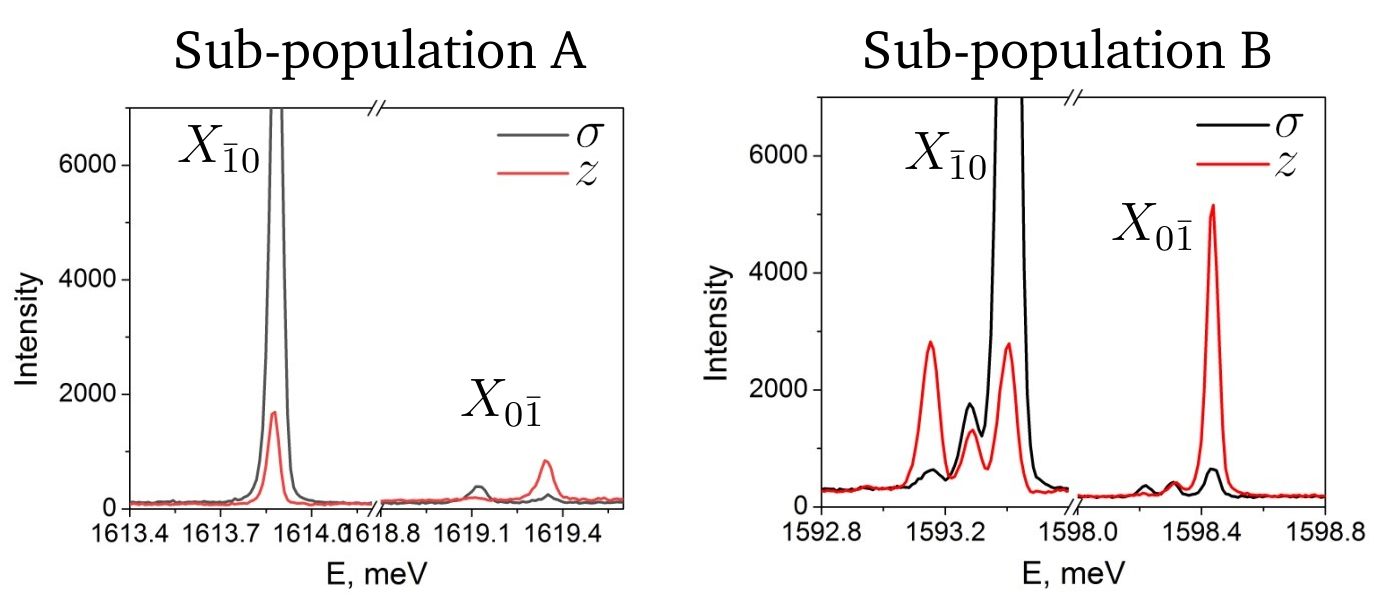
\includegraphics[width=\textwidth]{figures/single_neutral}
\end{center}
\caption{Spectra of two types of QDs in the neutral exciton decays. The $\sigma$ and $z$-polarised spectra are colour-coded black and red, respectively.\label{fig:single_neutral}}
\end{figure}

The negatively charged exciton spectra are shown in Fig. \ref{fig:single_negative}. Both hole types feature a single strong line in both $\sigma$ and $z$ polarisation. For $X_{0\bar{1}}$, this agrees with the predictions of all analysed groups. However, for $X_{0\bar{1}}$, the $z$-polarised peak seems to probe the bulk symmetry $T_d$, as $z$-polarised transitions are forbidden in the structure symmetry. However, Karlsson \textit{et al.} seem to have the $z$-polarised peak appear faintly, or not resolvable at all.
\\\hfill\\
\makebox[0pt][l]{%
\begin{minipage}{\textwidth}
\centering
    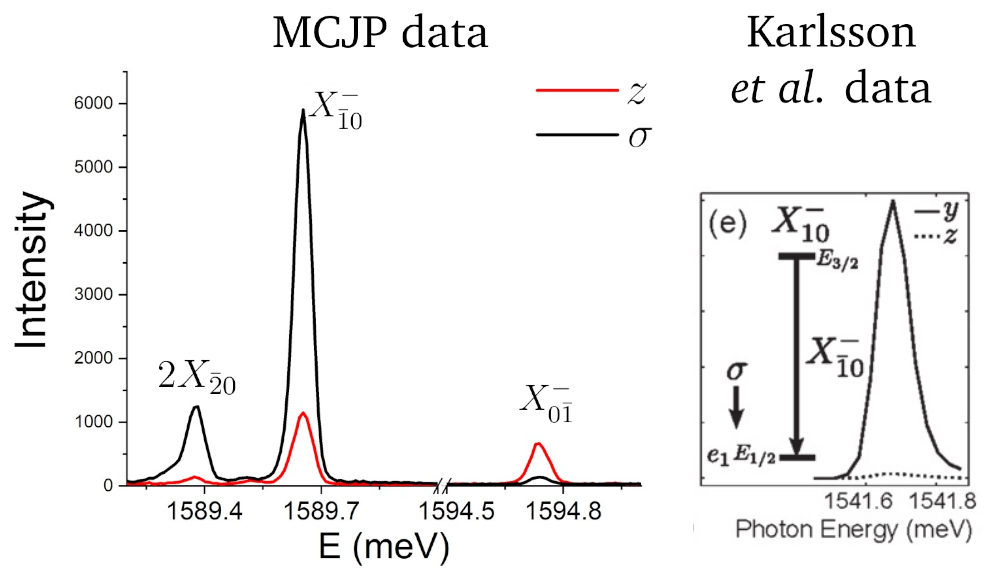
\includegraphics[width=.7\textwidth]{figures/single_negative_plus_karlsson}
 \captionof{figure}{Spectrum of the negatively charged excitons, compared between the new MCJP dataset and the Karlsson dataset. Karlsson dataset plot taken from \cite[Fig. 15 e)]{karlsson}}
 \label{fig:single_negative}
\end{minipage}
}\\\hfill\\

The spectra of positively charged excitons and biexcitons are shown in Fig. \ref{fig:exciton_positive}. For $2X^+_{\bar{2}1}$, 3 resolvable peaks with both $\sigma$ and $z$-polarised components are always present, with the latter polarisation contradicting the predictions of $C_{3v}$ and $D_{3h}$. In sub-population $A$ a fourth peak, with both $\sigma$ and $z$-polarised components, is usually present, but is not conclusively proven to be part of the complex by the MCJP correlation measurements. $4$ peaks in both polarisations would be good evidence for elevating to bulk symmetry.

For $X^+_{\bar{1}1}$, three peaks are always certain in both sub-populations, with $z$-polarised components seemingly weakened and multiple added faint $\sigma$-polarised peaks occuring in $B$. The three $z$-polarised peaks contradict $C_{3v}$ and $D_{3h}$ predictions and are consistent with $T_d$ for sub-population $A$, while the $4$ $\sigma$-polarised and $2$ resolvable $z$-polarised lines show agreement with $C_{3v}$ for sub-population $B$.

For $X^+_{1\bar{1}}$, four strong lines with both $\sigma$ and $z$ components are present for both types, contradicting $C_{3v}$ and $D_{3h}$ and agreeing with $T_d$. However, the relative intensities of lines $c,b,a$ disconfirm the assumption of emissions with no polarisation, since that predicts the $z$-polarised detector measuring the lines at half-intensity. Both populations here exhibit the dominance of the $z$-polarised component for lines $c$ and $b$. Altogether, this constitues weak evidence for elevation to the bulk symmetry, conditioned by the presence of another mechanism which introduces $z$-polarisation bias. Interestingly, in the Karlsson \textit{et al.} data, only two lines are detected in either polarisation, in agreement with both $C_{3v}$ and $D_{3h}$, contradicting the bulk symmetry elevation, for a subpopulation of $15\%$ of their QDs. Other QDs exhibited different spectra, typically with extra lines (\cite[Fig. 19]{karlsson}), which suggest partial elevation to $T_d$.
\\

\makebox[0pt][l]{%
\begin{minipage}{\textwidth}
\centering
    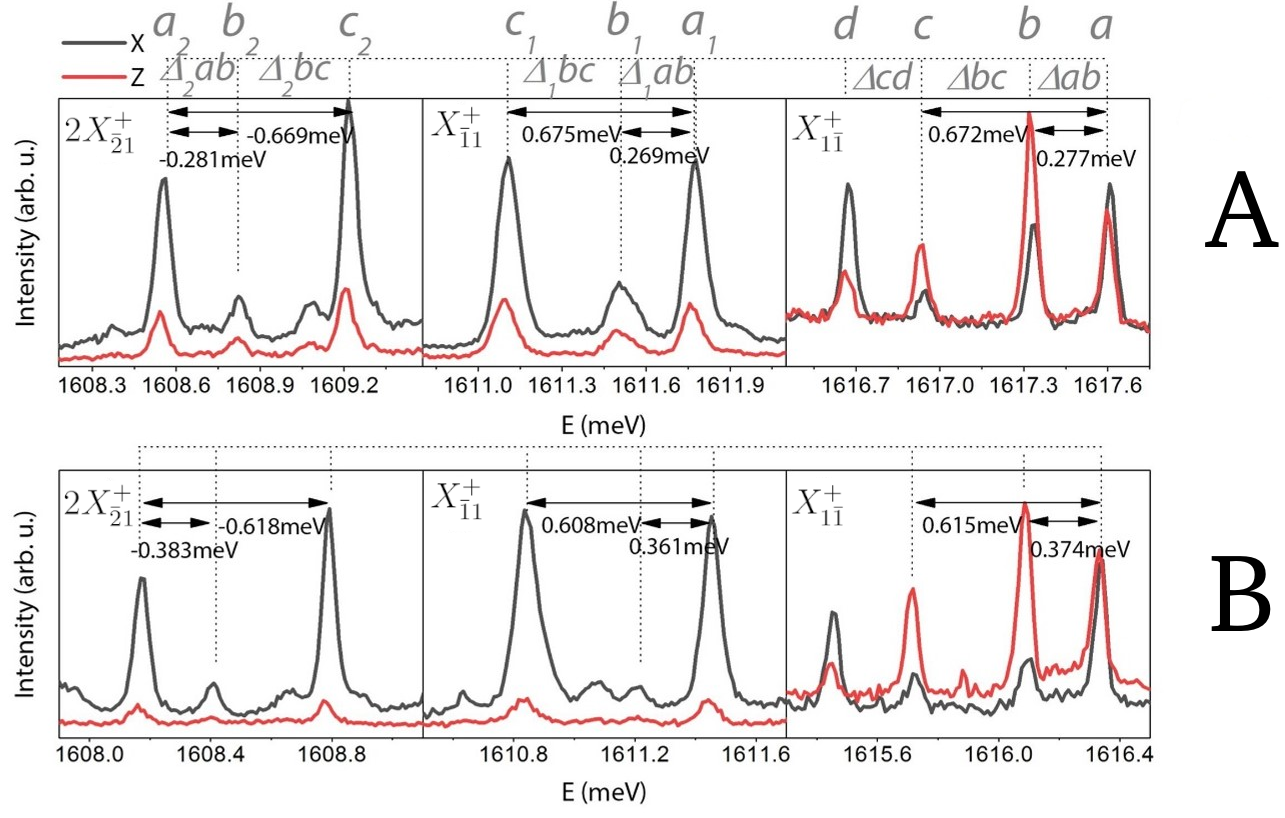
\includegraphics[width=0.9\textwidth]{figures/exciton_positive}
 \captionof{figure}{Spectrum of the positive biexciton $2X^+_{\bar{2}1}$ and the positive mixed-hole excitons $X^+_{\bar{1}1}$ and $X^+_{1\bar{1}}$. Two distinct sub-populations were identified, labelled $A$ and $B$. Major peaks are identified by MCJP and their energy differences highlighted.}
 \label{fig:exciton_positive}
\end{minipage}
}
\\\hfill\\

For other positively charged excitons and biexcitons, MCJP have no data. However, Karlsson \textit{et al.} identified a single line for either polarisation for $2X^+_{2\bar{1}}$, in agreement with $C_{3v}$ and disagreement with $T_d$. Similarly, $X^+_{1\bar{2}}$ had two $\sigma$-polarised lines and one $z$-polarised line, with another one predicted to overlap with a different peak, identified, in agreement with $C_{3v}$. For $X_{\bar{2}0}$, a single $\sigma$-polarised line was detected, seemingly in agreement with $C_{3v}$. However, activity in the $z$-polarised spectrum is faintly evident. Better-resolved measurement in the $z$-polarised spectrum could find evidence for weak elevation to the bulk symmetry.

The sectra of neutral biexcitons are shown in Fig. \ref{fig:biexciton_neutral}. MCJP were unable to conclusively identify all peaks in the $2X_{\bar{1}1}$ transition as belonging to it. Due to the ambiguous identification of lines and the unresolvability of the predicted large number of lines, the transition was not analysed here. Karlsson \textit{et al.} note that the $z$-polarised peaks may be present but very weak due to the heavy-hole recombination \cite[p. 16]{karlsson}, and thus missing $z$-polarised lines do not constitute evidence against elevation to $T_d$.

For the transition $2X_{\bar{2}0}$, a strongly resolvable $z$-polarised peak is measured, contradicting $C_{3v}$ and $D_{3h}$. While $T_d$ predicts $6$ $z$-polarised peaks, it is possible that they are too tightly spaced to be resolvable, especially since the energy splitting may be reduced due to the approximate nature of elevating to the bulk within symmetry suppression theory.

\makebox[0pt][l]{%
\begin{minipage}{\textwidth}
\centering
    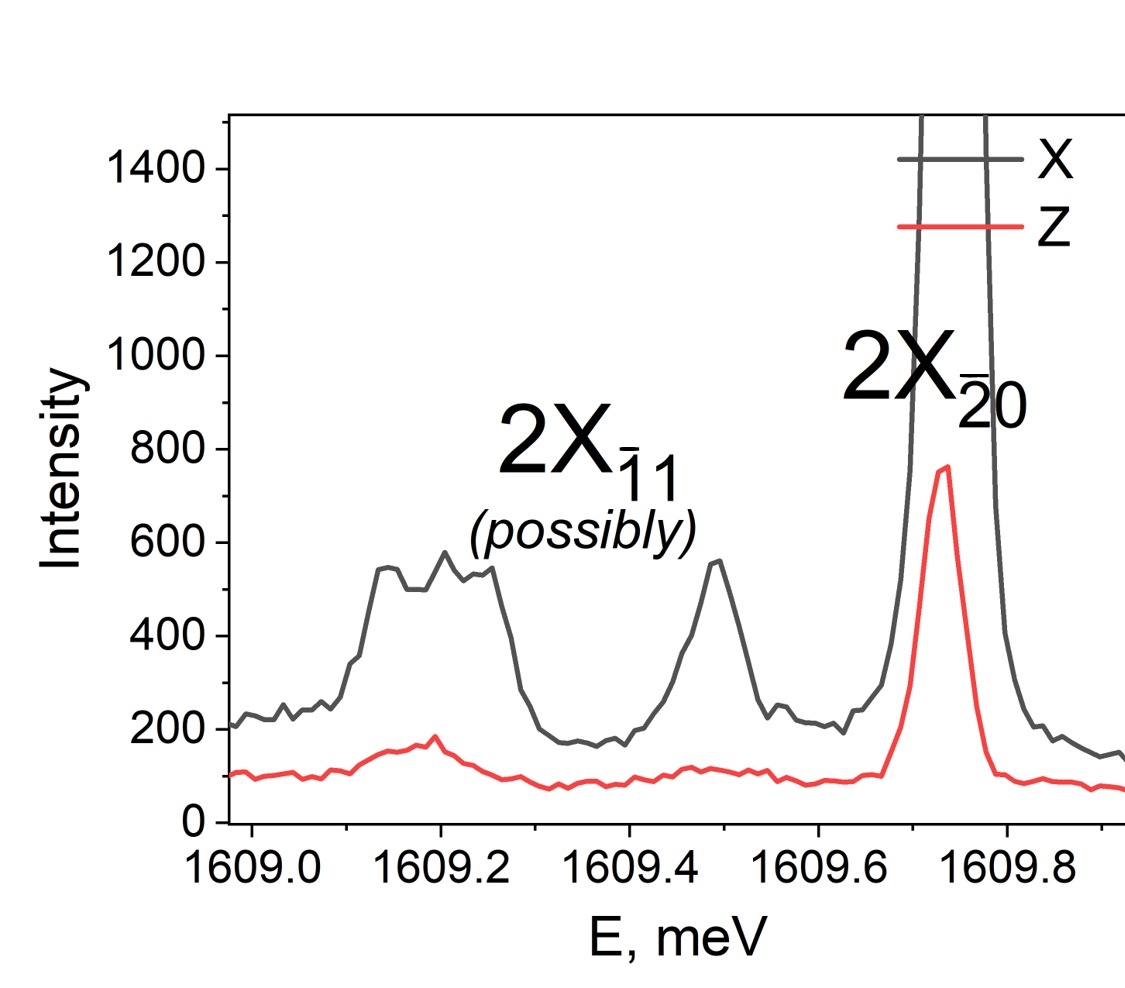
\includegraphics[width=.4\textwidth]{figures/biexciton_neutral}
 \captionof{figure}{Spectrum of two neutral biexcitons.}
 \label{fig:biexciton_neutral}
\end{minipage}
}